\documentclass[12pt]{jarticle}
\usepackage{a4wide}
\usepackage{amsmath}%数学記号
\usepackage{amssymb}%数学記号
\usepackage{epsfig}%図
\usepackage{latexsym}
\usepackage{supertabular}
\usepackage{graphicx}
\usepackage{color}
\usepackage{ascmac}
\usepackage{multicol}
\usepackage{ascmac}
\usepackage{systeme}
\usepackage{amsmath,cases}
\usepackage{float}
\usepackage{here}
\pagestyle{plain}

\newtheorem{theorem}{定理}[section]
\newtheorem{lemma}[theorem]{補題}
\newtheorem{proposition}[theorem]{命題}
\newtheorem{conjecture}[theorem]{予想}
\newtheorem{corollary}[theorem]{系}
\newtheorem{definition}[theorem]{定義}
\newtheorem{example}[theorem]{例}
\newtheorem{exercise}[theorem]{例題}
\newtheorem{problem}[theorem]{問}
\newtheorem{algorithm}[theorem]{アルゴリズム}
\newtheorem{remark}[theorem]{注意}

\def\qed{{\hfill$\square$}}
\def\proof{{\vspace{-0.3cm}f 証明: \,}}
\def\solution{{\vspace{-0.3cm}f 解: \,}}
\def\N{{\Bbb N}}
\def\Z{{\Bbb Z}}
\def\Q{{\Bbb Q}}
\def\R{{\Bbb R}}
\def\C{{\Bbb C}}
\def\F{{\Bbb F}}
\def\D{{\mathcal D}}
\def\mod{{\mathrm{mod\,\,}}}
\def\GL{{\mathrm{GL}}}
\def\GF{{\mathrm{GF}}}
\def\H{{\mathcal{H}}}

\setlength{\textwidth}{170mm}
\setlength{\textheight}{240mm}
\setlength{\oddsidemargin}{-5mm}
\setlength{\evensidemargin}{-5mm}
\setlength{\topmargin}{-10mm}
\setlength{\headheight}{0mm}
\setlength{\headsep}{10mm}

\title{項目反応理論}
\begin{document}
\maketitle
\section{実験}
\subsection{概要}
教職教養に関する問題を$8$問出題し、その回答を項目特性図によって、誤答分析した後に、各選択肢をみて正答分析を行ってみる。
\subsection{条件設定}
教職教養に関する問題ということで、なるべくこれに関して勉強を行っているほうがよいと考え、教育学部に在籍しているもしくは在籍していたもの$30$人を対象に行った。出題する問題は、教職教養の勉強に広く用いられる時事通信社の「教職教養の演習問題」から$8$題出題する。
\subsection{問題に関して}
第$1$問、第$2$問は教育史から出題した。出題された文に関する人物を選ぶ問題である。第$1$問は第$2$問に比べて比較的基礎的な問題と予想されるので、項目特性曲線は、$G$型になると予想される。一方で、第$2$問は九州の中の県では、あまり出題されない日本教育史であるため、正答率は群に関係なく低くなるD型になると予想される。

第$3$問は教育原理から出題した。難易度は高く設定された問題である。理由としては、一見したら全部正しいように見えるが、実は間違っているのはコメニウスはアメリカの学者ではなくチェコの学者であるという点である。これは実際に出された問題であり、ほとんど消去法で国の違いにたどり着くか、運で正答するかという問題である。このことを考えると$M$型になると予想できる。

第$4$問、第$5$問は教育法規から出題した。第$4$問は、正解の選択肢以外はほとんど間違いようのない選択肢ばかりである。つまりどの群においても正答率は高くなると考えられるので、$E$型になると予想される。第$5$問は難易度は比較的簡単に設定されている。しかし、$2$択までは簡単に絞れるがそこからしっかりと正答を導けるのかが大事になってくる問題である。このことから、高位群では安定の正答率が出て、下位群になればなるほど不安定になると考えられる。よって。$H$型になると予想される。

第$6$問、第$7$問、第$8$問は、教育心理から出題した。第$6$問は問題文が理解しづらい問題である。選択がバラバラになると考えられるため、$M$型になると予想される。第$7$問、第$8$問は、記憶していればしっかりと答えられる問題である。
\section{項目特性図とは}
項目特性図について復習しておく。項目特性図とは、(流儀は多々あるが今回は)横軸に能力特性で分けられた群番号、縦軸には郡ごとの正答率を付したグラフである。グラフの形によっていくつかの型に分けられた。ここで、能力特性で群に分けるとは合計得点をもとに高いものから$5$群、低い者たちを$1$群とし振り分けることである。型については以下の通りである。%ゼミプリントから持ってくる
\begin{itembox}[l]{型の復習}
  \begin{itemize}
    \item[G型]  高識別力項目\\最下位群から高位群にかけて急激に正答率が上がっている項目
    \item[L型]  下位識別力項目\\下位群は正答率が非常に低く、そこから中位群にむけて正答率が高くなり、それ以降は高い正答率で安定する項目
    \item[H型]  上位識別力項目\\中位群までは安定的に正答率が低く、そこから正答率が急激に上昇する項目
    \item[E型]  高通過率項目\\正答率のグラフが高位から始まり全体的に高位に張り付いている項目
    \item[M型]  中通過率項目\\テスト得点の高い者、低い者も正答率が変わらない項目
    \item[D型]  低通過率項目\\正答率が全体的に低位に張り付いている項目
    \item[B型]  右下がり項目\\上位群より下位群の方が正答率が高い項目
  \end{itemize}
\end{itembox}
\newpage
\section{正答分析}
第$1$問目について、グラフは以下の通りになった。
\begin{figure}[H]
  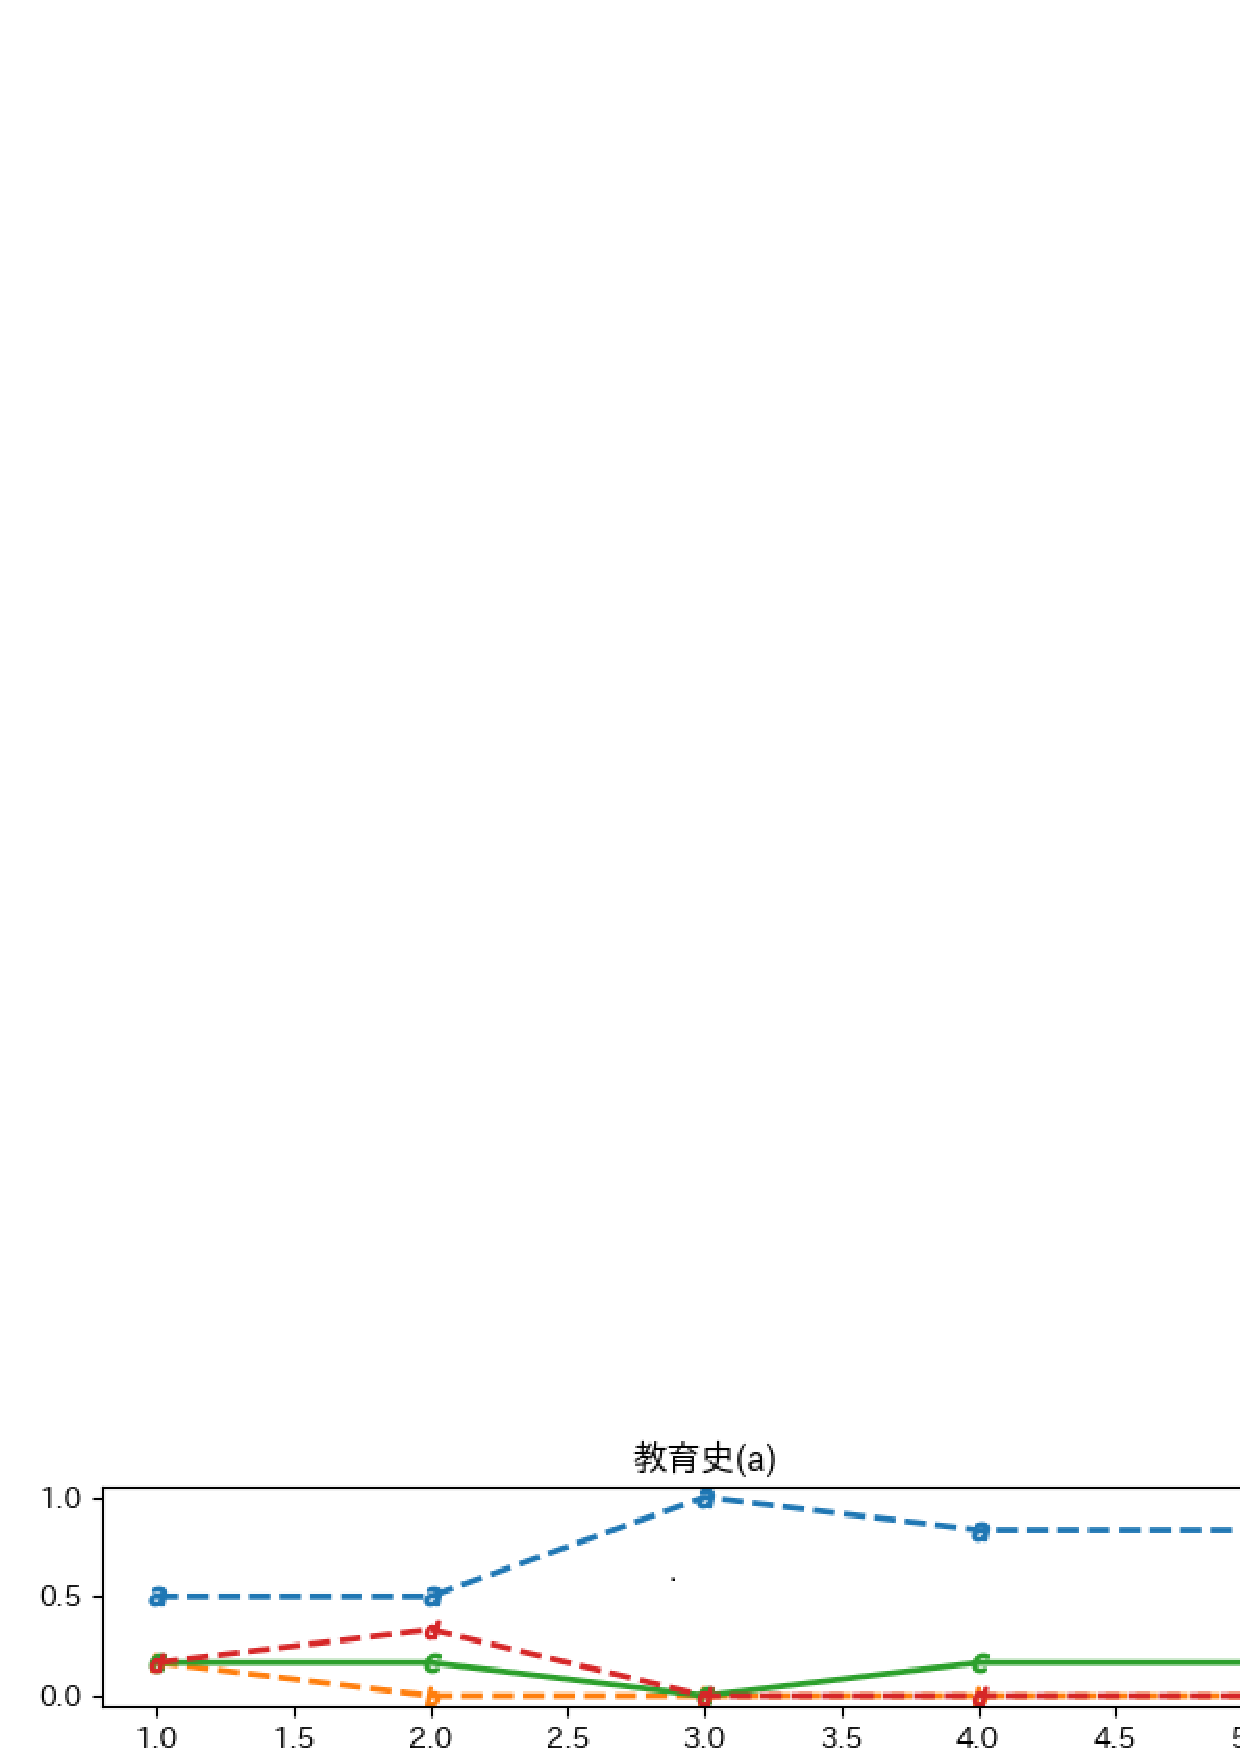
\includegraphics[bb = -7 60 1 1,scale = 1.5]{Figure_1.png}
\end{figure}
\leavevmode \\
\\
\\
\\
\\
\ \ 正答率は中位群までは上昇していて、上位群では多少差はあるが高い正答率を有している。$L$型に近いグラフをしている。

第$2$問目について、グラフは以下の通りになった。
\begin{figure}[H]
  \includegraphics[bb = -7 60 1 1,scale = 1.5]{Figure_2.png}
\end{figure}
\leavevmode \\
\\
\\
\\
\\
\ \ 下位群から中位群までは正答率は低いが、そこから上位群にかけて急激に上昇している。$1$問目より$L$型のグラフをしている。

第$3$問目について、グラフは以下の通りになった。
\begin{figure}[H]
  \includegraphics[bb = -7 60 1 1,scale = 1.5]{Figure_3.png}
\end{figure}
\leavevmode \\
\\
\\
\\
\\
\ \ 下位群から上位群に行くにつれて順当に正答率が上がっている。グラフは$G$型と言える。

第$4$問目について、グラフは以下の通りになった。
\begin{figure}[H]
  \includegraphics[bb = -7 60 1 1,scale = 1.5]{Figure_4.png}
\end{figure}
\leavevmode \\
\\
\\
\\
\\
\ \ 正答率はどの群も安定して$6$割を超えて最上位群は正答率が$1$である。グラフは$E$型に近い。

第$5$問目について、グラフは以下の通りになった。
\begin{figure}[H]
  \includegraphics[bb = -7 60 1 1,scale = 1.5]{Figure_5.png}
\end{figure}
\leavevmode \\
\\
\\
\\
\\
\ \ 正答率は全体的に高位に張り付いている。$4$問目より$E$型である。

第$6$問目について、グラフは以下の通りになった。
\begin{figure}[H]
  \includegraphics[bb = -7 60 1 1,scale = 1.5]{Figure_6.png}
\end{figure}
\leavevmode \\
\\
\\
\\
\\
\ \ 正答率は下位群から中位群にかけては上昇しており、上位群では安定した正答率を有している。

第$7$問目について、グラフは以下の通りになった。
\vspace{0.5cm}
\begin{figure}[H]
  \includegraphics[bb = -7 60 1 1,scale = 1.5]{Figure_7.png}
\end{figure}
\leavevmode \\
\\
\\
\\
\\
\ \ $5$問目と似ていて正答率は全体的に高位に張り付いている。$E$型である。

第$8$問目について、グラフは以下の通りになった。
\vspace{0.5cm}
\begin{figure}[H]
  \includegraphics[bb = -7 60 1 1,scale = 1.5]{Figure_8.png}
\end{figure}
\leavevmode \\
\\
\\
\\
\\
\ \ 下位群から上位群に行くにつれて順当に正答率が上がっている。グラフは$G$型と言える。
\section{誤答分析}
$1$問目に関して、$G$型になると予想したが実際は少し$L$型に近いグラフが得られた。また$2$問目に関しては$D$型になる予想だった。問題文は以下のとおりである。\\
\hrulefill
\vspace{3cm}
\begin{figure}[H]
  \includegraphics[bb = -7 60 1 1,scale = 0.4]{ques_1.png}
\end{figure}
\hrulefill\\
$1$問目は比較的どの自治体にも出題される問題である。正解である他では$(3)$のシュプランガーが選ばれている。しかし、正答率から$2$択までは絞れており、確信をもって正解を選択できなかった者が下位群には少し多かったと考えられる。$2$問目は、九州ではほとんど出題されることのない日本教育史の問題である。これはほぼ運で正解者がでたりでなかったりすると考え、$D$型になる予想だった。しかし、グラフは$L$型に近いものだった。しかし誤答を見てみると正解の選択肢以外はほぼすべて偏りなく選ばれているので、予想としては当たっていると考えた。

$3$問目の問題文は以下のとおりである。\\
\hrulefill
\vspace{4.5cm}
\begin{figure}[H]
  \includegraphics[bb = -7 60 1 1,scale = 0.4]{ques_2.png}
\end{figure}
\hrulefill\\
この問題に関しても、先ほどの問題と同じようにほぼ運で正解者がでたりでなかったりすると考えたがグラフは$G$型に近く、誤答も$(b)$と$(d)$が下位群には圧倒的に選ばれる結果となった。$(a)$について、これは考えてみると特別支援学校がない県はなさそうであるので除外される。この手の選択肢は、いろいろな役職や事項が盛り込まれていて細かく記憶している必要があるので正解なのか不正解なのかわかりにくくなっている。$(d)$は国のいじめ防止基本方針によって定められたものであるが、被験者の数名に話を聞くと、出題される時は「少なくとも$3$ヶ月」ではなく、「相当期間(少なくとも$3$ヶ月)」と表記されることが多いとわかった。細かく覚えていることによってこの選択肢を選んでしまったのだと考えらる。

$4$問目の問題文は以下のとおりである。\\
\hrulefill
\vspace{4.5cm}
\begin{figure}[H]
  \includegraphics[bb = -7 60 1 1,scale = 0.4]{ques_3.png}
\end{figure}
\hrulefill\\
選択肢$(a)$はすべての群でほとんど選ばれることはなかったので、機能してないことがわかる。

$5$問目の問題文は以下のとおりである。\\
\hrulefill
\vspace{3cm}
\begin{figure}[H]
  \includegraphics[bb = -7 60 1 1,scale = 0.4]{ques_4.png}
\end{figure}
\hrulefill\\
この問題に関して作問の意図として、義務教育と普通教育の$2$択で迷ってほしい、というのがあると考えられる。しかし、正解の選択肢以外はほぼ機能していないことがわかる。

$6$問目から$8$問目までの問題文は以下のとおりである。\\
\hrulefill
\vspace{6.5cm}
\begin{figure}[H]
  \includegraphics[bb = -7 60 1 1,scale = 0.4]{ques_5.png}
\end{figure}
\hrulefill\\
$6$問目$7$問目に関しては下位群では誤答も少しばらけているが、中位群から上位群にかけては、正解以外の選択肢はしっかりと除外されている。$8$問目は、比較的どの群でも正解の選択肢以外が機能していることがわかる。
\section{まとめ}
今回は$30$人を対象に実験を行ってみたが、実際の学校で運用することを考えるともっとデータが取れるのでより精度を高くできると感じた。しかし、いじめに関する問題のように、選択した理由などを直接聞いて原因を究明するのは少し難しくなると感じた。学校単位で行えば、クラスの傾向、学年としての傾向など分けて考えることもできそうである。私自身の専門である数学のテストで運用していくためには与える選択肢をしっかりと考える必要がある。例えば、間違えやすい計算のところで間違える想定の選択肢などがあげられそうである。今回は、運用のテストだったので次回は、数学の問題で行ってみたい。また、ロジスティックモデルの$ICC$を用いた分析にも挑戦したい。






\end{document}
